% #############################################################################
% This is Chapter 3
% !TEX root = ../main.tex
% #############################################################################
% Change the Name of the Chapter i the following line
\fancychapter{Architecture of the Optimization Framework}
% The following line allows to ref this chapter
\label{chap:architecture}

This dissertation focuses on the study of optimization algorithms that are able to more efficiently handle a set of problems involving time-consuming functions. Apart from the theoretical study and literature review, this dissertation proposes a general-purpose framework to enable the application of different types of optimization algorithms, both for \ac{SOO} and \ac{MOO} problems. The concretization of such framework requires: (1) the definition of an abstraction layer, that enables the modeling of optimization problems, (2) a wide variety of optimization algorithms to address different optimization problems, (3) a set of performance indicators to provide the user with a measure of the algorithms' quality when testing multiple algorithms, and (4) visual representations of the obtained results to provide more comprehensive feedback over the optimization results. ~\Cref{fig:solution} shows the  solution's different components and its external connections.

\begin{figure}[htbp]
	\centering
	%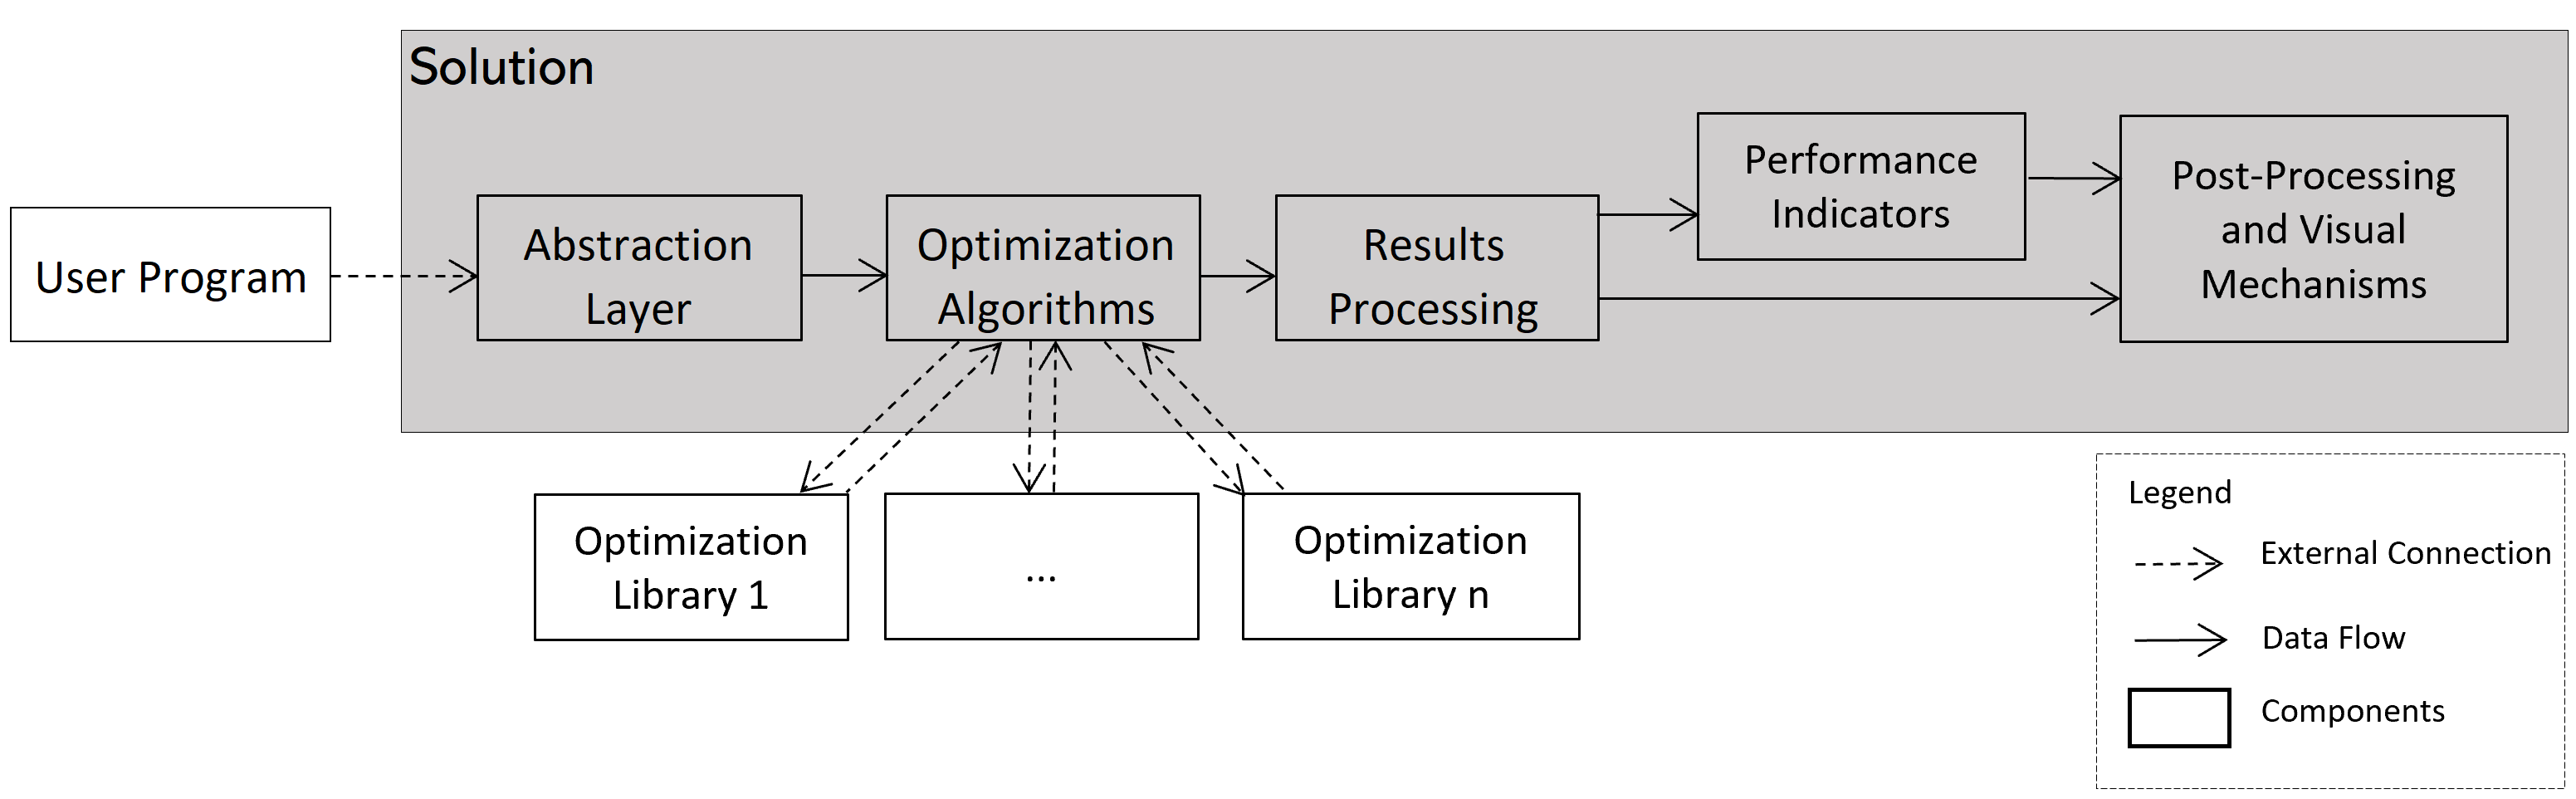
\includegraphics[width=\textwidth]{./Images/Solution/solution_architecture_2.PNG}
	%\caption{Architecture of the solution.}
	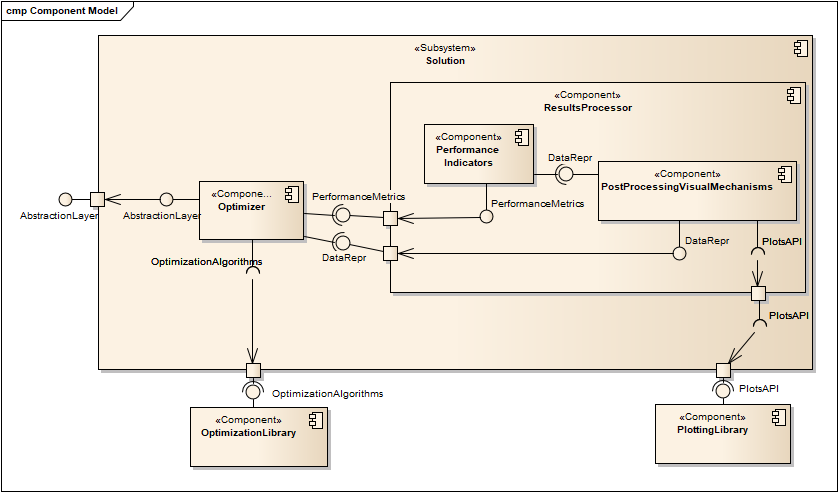
\includegraphics[width=\textwidth]{./Images/Solution/ComponentModel3.png}
	\caption{Components diagram of the solution.}
	\label{fig:solution}
\end{figure}

With the aforementioned framework, users are able to address optimization problems involving time-intensive functions, for which the objective functions' analytical forms are unavailable. In order to verify its executability and suitability for conducting multiple optimization processes, we developed a prototype of such framework. This chapter describes the main components of the developed framework and also the main requirements that led to their implementation. 


\section{Programming Language}
\todo{Não dar tanto detalhe? Parecer que é uma escolha secundária.}
One of the first concerns when developing the framework was the programming language to use. The currently implemented framework uses two programming languages, which were chosen based on the available optimization libraries, the domain of the solution, and the performance of each programming language.
 
On the one hand, several languages already provide well-known optimization libraries, which have been tested, and independently validated. As a result, instead of attempting to implement the optimization algorithms again, we sought for programming languages which provided easy access to these implementations. On the other hand, because we are dealing with optimization algorithms that involve numerical computations, we aimed at languages which provided fast numeric computation without the need to dive into lower level languages, such as C or Fortran. Finally, we also considered the performance of the programming language and the mechanisms provided by the language to make code development more efficient (e.g., avoiding boilerplate code).

To develop the optimization framework, we used Julia\footnote{https://julialang.org}, a recent programming language that has been shown to be very promising in the numerical optimization domain, and that provides mechanisms to speed code development (e.g., functional programming paradigm, macros). Despite having a smaller library's repository than, for instance, Python\footnote{https://www.python.org/}, Julia has grown to implement some of Python's optimization libraries (e.g., Scikit-learn, NLopt), and, therefore, also provides some of the functionalities of Python.   

Unfortunately, Julia is a recent language and, whilst some of these libraries can effectively become more efficient in Julia (e.g., Scikit-learn), other libraries present some limitations regarding the supported functionalities. For instance, in terms of data processing and visualization, Python presents a more stable  and better documented set of libraries (e.g., Pandas, Seaborn, Matplotlib, Plotly). For all these reasons, in order to facilitate the processing and visualization of the optimization results, we adopted Python as the second programming language.

% Furthermore, the data transfer between Julia and Python is easily achieved by using the mechanisms provided by Julia (e.g., macros) and a wrapper library, PyCall. \todo{Nao sei muito bem como melhorar isto.. Mas o vocabulario está um bocado simplorio...}

One aspect to take into consideration is that, albeit being implemented in Julia and Python, our solution could have been implemented in other programming languages such as Java or C++, which also provide several optimization and data processing libraries. In this dissertation and as it will be explained in ~\cref{chap:implement,chap:evaluation}, we had the extra motivation that the case studies were already developed in Julia. Thus, by creating an abstraction layer in Julia, we were able to easily integrate optimization processes with an existing algorithmic design tool for architectural projects, and to easily test the effectiveness and quality of the proposed solution within the architectural context. 

\section{Abstraction Layer}
The abstraction layer is designed to abstract the user from the logic of other external optimization tools. By providing a uniform \ac{API}, this abstraction layer eliminates the apparent chasm between different optimization tools and facilitates the use of algorithms from different optimization libraries, incurring no additional efforts for the user, i.e., the user is not required to make any further modifications to the program (e.g., changing the program structure, changing the primitive operations, in order to test different optimization algorithms). 

To define such abstraction layer, one alternative is to adopt a currently available domain-specific modeling language for optimization (e.g., JuMP, PyOMO, MultiJuMP, PISA, AMPL). Not only would this allow users to have access to well-tested and more stable \acp{API}, but they would also have out-of-the-box access to a wide variety of optimization solvers capable of handling various problems. 

Notwithstanding their benefits, the abstraction layer provided in this dissertation does not make use of these modeling languages due to (1) their lack of support for both \ac{SOO} and \ac{MOO} problems, (2) complexity of syntax rules and need for deep understanding of the language to use it, and (3) lack of solvers or mechanisms that enable the execution of optimization solvers capable of efficiently addressing optimization problems involving costly simulation-based evaluation functions. As a result, to explore one of these modeling languages would require not only additional developments to create the mechanisms to support both \ac{SOO} and \ac{MOO} problems, but also to create a new solver capable of addressing the specific type of problems that this dissertation set out to address. 

Nevertheless, influenced by existing optimization modeling languages, the abstraction layer's operations remove the complexity associated to most modeling languages and allow users to incrementally combine them in order to model more complex optimization problems. Moreover, the abstraction layer is designed to enable the execution of any of the optimization approaches discussed in~\cref{sec:optimizationproblems}, ranging from \ac{SOO} to \ac{MOO} approaches, passing through the design of experiments approach.

\begin{lstlisting}[caption={Simple example of the framework's API.},label=juliaCode]
# Analytical Objective Functions
f1(x) = x^2
f2(x) = (x - 2)^2

let var1 = RealVariable(-10, 10),
	obj1 = Objective(f1, :MIN),
	obj2 = Objective(f2, :MIN),
	model = Model([var1], [obj1, obj2])
  solve(NSGAII, model, max_evals=100) 
end
\end{lstlisting}

\todo{BF - este parágrafo quebra totalmente a leitura. A transição é super brusca em relação ao anterior. }
As described in \cref{chap:back}, the definition of an optimization process is composed of two parts: the modeling of the optimization problem and the optimization algorithm. This \ac{API} provides not only primitives to define variables, objective functions, and, when necessary, constraints, but also empowers users with the ability to use and fine-tune the parameters of each optimization algorithm, i.e., parameters that control the detail of the search process. The entire \ac{API} is intuitive and simple to use by less experienced users, but flexible to be extended and improved by programmers, which may decide to add more algorithms or integrate other optimization libraries. \Cref{juliaCode} illustrates how to use the framework's \ac{API} to model a bi-objective unconstrained optimization problem. To this end, in order to solve the problem, the user needs to: (1) create the model of the problem (\textit{line 8}), which requires the definition of the variables (\textit{line 5}) and the objective functions (\textit{lines 1-3 and 6-7}); (2) to specify the optimization algorithm (\textit{line 12}), which in this case is the \ac{NSGA-II}; and (3) the maximum number of costly evaluations during the optimization search (\textit{line 12}).


\section{Optimization Algorithms}
\label{sec:optalgos}

Optimization algorithms represent a crucial part in an optimization process and, consequently, in the developed solution. In order to study different optimization algorithms and to test their suitability for specific optimization problems~\cite{Wolpert1997NFLT}, a large set of distinct and representative optimization algorithms should be provided. In addition to diversity, our solution also provides the users with the flexibility to configure the different parameters associated to the optimization algorithms, commonly known as hyperparameters. By fine-tuning the values of these hyperparameters for a specific problem, the performance of optimization processes can be drastically improved. 

Another important requirement that is taken into consideration is that at least a subset of the provided algorithms must be tailored to address optimization problems that incorporate time-consuming evaluation functions, and for which information is difficult to obtain. To address this requirement, we reviewed the most reputed \ac{SOO} and \ac{MOO} open-source derivative-free optimization libraries. After a thorough analysis of different optimization libraries, the final solution presents a total of 36 algorithms from 4 different libraries, listed in \cref{table:algorithms}. 

\begin{table}[]
	\centering
	\begin{tabular}{cccll}
		\rowcolor[HTML]{EFEFEF} 
		\textbf{Class} & \textbf{Objectives} & \textbf{Global} & \textbf{Algorithm} & \textbf{Library} \\ \hline
		& Both & G & Full-factorial & None \\
		& Both & G & Latin Hypercube & None \\
		& Both & G & Random & None \\
		\multirow{-4}{*}{Sampling} & Both & G & Stratified Random & None \\ \hline
		& S & G & CRS2 & NLopt \\
		& M & G & CMA-ES & Platypus \\
		& S & G & ESCH & NLopt \\
		& M & G & ES & Platypus \\
		& M & G & $\epsilon$-MOEA & Platypus \\
		& S & G & GA & Platypus \\
		& M & G & GDE3 & Platypus \\
		& M & G & IBEA & Platypus \\
		& S & G & ISRES & NLopt \\
		& M & G & MOEAD/D & Platypus \\
		& M & G & NSGA-II & Platypus \\
		& M & G & NSGA-III & Platypus \\
		& M & G & PAES & Platypus \\
		& M & G & PESA2 & Platypus \\
		& M & G & SPEA2 & Platypus \\
		& M & G & OMOPSO & Platypus \\
		\multirow{-17}{*}{Metaheuristic} & M & G & SMPSO & Platypus \\ \hline
		& S & G & DIRECT & NLopt \\
		& S & G & DIRECT-L & NLopt \\
		& S & L & NMS & NLopt \\
		& S & L & PRAXIS & NLopt \\
		\multirow{-5}{*}{Direct search} & S & L & Subplex & NLopt \\ \hline
		& S & L & BOBYQA & NLopt \\
		& S & L & COBYLA & NLopt \\
		& Both & G & Decision Tree & Scikit-learn \\
		& Both & G & GP & Scikit-learn \\
		& Both & G & Linear & Scikit-learn \\
		& Both & G & MLP & Scikit-learn \\
		& Both & G & Random Forest & Scikit-learn \\
		& Both & G & RBF-Cubic & pySOT \\
		& Both & G & RBF-Linear & pySOT \\
		\multirow{-10}{*}{Model-based} & S & G & SVR & Scikit-learn
	\end{tabular}
	\caption[Solution's list of supported algorithms]{List of the currently available algorithms in the implemented solution, discriminated by class, number of objectives, aim of the search, and the optimization library implementing it. Note: L - Local, G - Global, M - Multi, S - Single.}
	\label{table:algorithms}
\end{table}

To implement sampling algorithms, the framework makes use of Julia's arrays and random primitives, requiring no additional libraries to be implemented. Secondly, by integrating the NLopt~\cite{NLOPT} library within our framework\footnote{A special thank you to Guilherme Ilunga who contributed to this integration.}, we were able to expose 10 \ac{SOO} algorithms and, thus, to test algorithms from the three derivative-free optimization classes. Moreover, this library has already been used in Goat, an architectural design optimization tool, which has been applied in some architectural studies as well~\cite{Wortmann2017ADO}. Thirdly, the Platypus library~\cite{platypus} was chosen from a set of \ac{MOO} libraries, that included Platypus, jMetal~\footnote{http://jmetal.github.io/jMetal/}, MOEAFramework~\footnote{http://moeaframework.org/}, Paradiseo~\footnote{http://paradiseo.gforge.inria.fr/}, and PaGMO~\footnote{https://esa.github.io/pagmo2/}. The Platypus library was the final choice due to the variety and quality of the \ac{MOO} algorithms provided, the ease of integration with the Julia programming language, and the cleanness and readability of its \ac{API}. Finally, the last integrated library was Python's Scikit-learn~\cite{scikit-learn}, which provides the basis algorithms for constructing more complex model-based algorithms, both for \ac{SOO} and \ac{MOO} problems.

When providing a framework that interfaces multiple libraries, it is important that the \ac{API} remains simple, abstracting the user from the different logic associated with the integrated libraries. To this end, the developed framework exposes a single and unified \ac{API}, enabling users to easily apply algorithms from different libraries and requiring no additional efforts or modifications (e.g., change the invocation method, change the name of parameters) from the user. Additionally, in order to extend the currently framework with other optimization algorithms, the programmer is only required to implement a connector between the proposed \ac{API} and the optimization library's \ac{API}.

\section{Performance Indicators}
%One of the goals of this thesis is to compare different optimization algorithms and assess the influence of their inherent mechanisms and assumptions in the overall performance of optimization processes. To this end, it is necessary to have a simple way of verifying the quality of these algorithms. 
Regarding the performance indicators, our solution enriches the abstraction layer previously discussed with a set of quality indicators for algorithms. While for comparing \ac{SOO} algorithms, these indicators usually resume to discovering both the value of the best found solution and the number of evaluations (or time) required to reach that value, for comparing \ac{MOO} algorithms this solution implements a subset of the indicators discussed in \cref{ssec:performance}, namely, the unary indicators \ac{ONVG}, \ac{ONVGR}, spacing, spread, maximum spread, \ac{ER}, \ac{GD}, \ac{HV}, and \ac{IGD}, and the binary indicators R-metrics, $\epsilon$ indicators, and the two set coverage.

Notwithstanding the utility of quantitatively qualifying the performance of different algorithms, this information can be difficult to interpret by less experienced users. To enhance interpretability, the proposed solution introduces post-processing and visualization functionalities discussed in the following section.

\section{Visual and Post-Processing Mechanisms}
In the architectural context, where architects often lack knowledge about optimization, visual and post-processing mechanisms become very important to promote a better comprehension and enable the making of more informed decisions. 

%  Why do we want visual and post-processing mechanisms ?  Why is it important? 
Often disregarded by optimization tools, the possibility to choose one of the best found solutions is highly advantageous. On the one hand, it allows users to examine the solutions and to choose the one that better fits their needs. As an example, consider the optimization of a specific aspect of a building design. It is often the case that the solution returned by the optimization algorithm is not the preferred solution, either because of more subjective opinions or, in some cases, because the best solution for that aspect might negatively impact other aspects which are not being considered (e.g., increasing the daylight illuminance often has repercussions on the thermal conditions and on the energy consumptions of a building). One other use case is the ability to examine different equally optimal solutions, particularly useful when handling multi-modal problems, for which there can be distinct solutions that yield the same optimal value. Unfortunately, many optimization tools obliterate most of these solutions, only providing the user with one solution. On the other hand, sometimes close to optimal solutions suit the user intentions better. By providing both optimal and close to optimal solutions, users would be empowered with a better understanding of optimization results, which can help them make more informed decisions. 

% How does our solution improves this?
The framework developed in this dissertation uses Python's data processing and visualization libraries, including, Pandas, Scikit-learn, Matplotlib, Seaborn, and Plotly to produce post-processing and visualization scripts that can be interpreted and manipulated by users to enrich the information obtained from optimization processes. By providing a simple way of visualizing the results in different layouts (e.g., statistics, distribution, correlations, parallel coordinate graphs, Pareto front, convergence graphs) and for post-processing them (e.g., outliers removal, interpolation of results), users are able to better understand the optimization process. 

Moreover, unlike most existing optimization tools, our solution offer out-of-the-box mechanisms to provide traceability and predictability about optimization processes. The solution preserves information regarding the configurations (e.g., model of the optimization problem, algorithm parameters) and the optimization results in files, which are updated during the course of the optimization process. 

To further take advantage of these files, our solution exposes a set of primitives in the abstraction layer that allows the reuse of optimization result files by providing them as input data for other optimization algorithms. This feature can be particularly relevant when testing different optimization algorithms in problems involving time-consuming simulation-based evaluation functions, as it reduces the overall optimization computational time.

% Using these files, we are able not only to input them to other post-processing tools (e.g., visualization, statistics), but also to hot start and pause/resume optimization processes.

% Limitations
Although the implemented framework does not provide real-time data information about the current state of the optimization process, our framework can be easily extended to include those features, since it rests on a fortified mechanism of real-time logging, that preserves both the configurations and the results involved in the optimization process. Additionally, because the framework updates these files with new information in real-time, the user is able to visualize the most recent information if he reruns the visual mechanisms again. With this feature users are able to examine in real-time the solutions that have already been evaluated by the optimization process, and decide if any of the found solutions already fulfils their intentions, or if they should wait for the optimization process to finish. 

To promote early decisions regarding an optimization process, our framework provides the user the ability to define functions to process different solutions (e.g., obtain other relevant information about the solution, communicate the values to other tools), which are then associated as callbacks to the visual outputs. Upon selecting a certain solution, these functions are triggered, thus executing the behavior previously defined by the user. \Cref{fig:interactivefeature} shows a possible application of this feature within the architectural practice, where the user selects the first optimal solution on the graph, represented by a black square, and the corresponding callback function is executed. In this case, the callback function used the values of the parameters associated to the selected solution to generate the corresponding 3D model of a  design in a 3D modelling tool. 

\begin{figure*}[htbp]
	\centering
	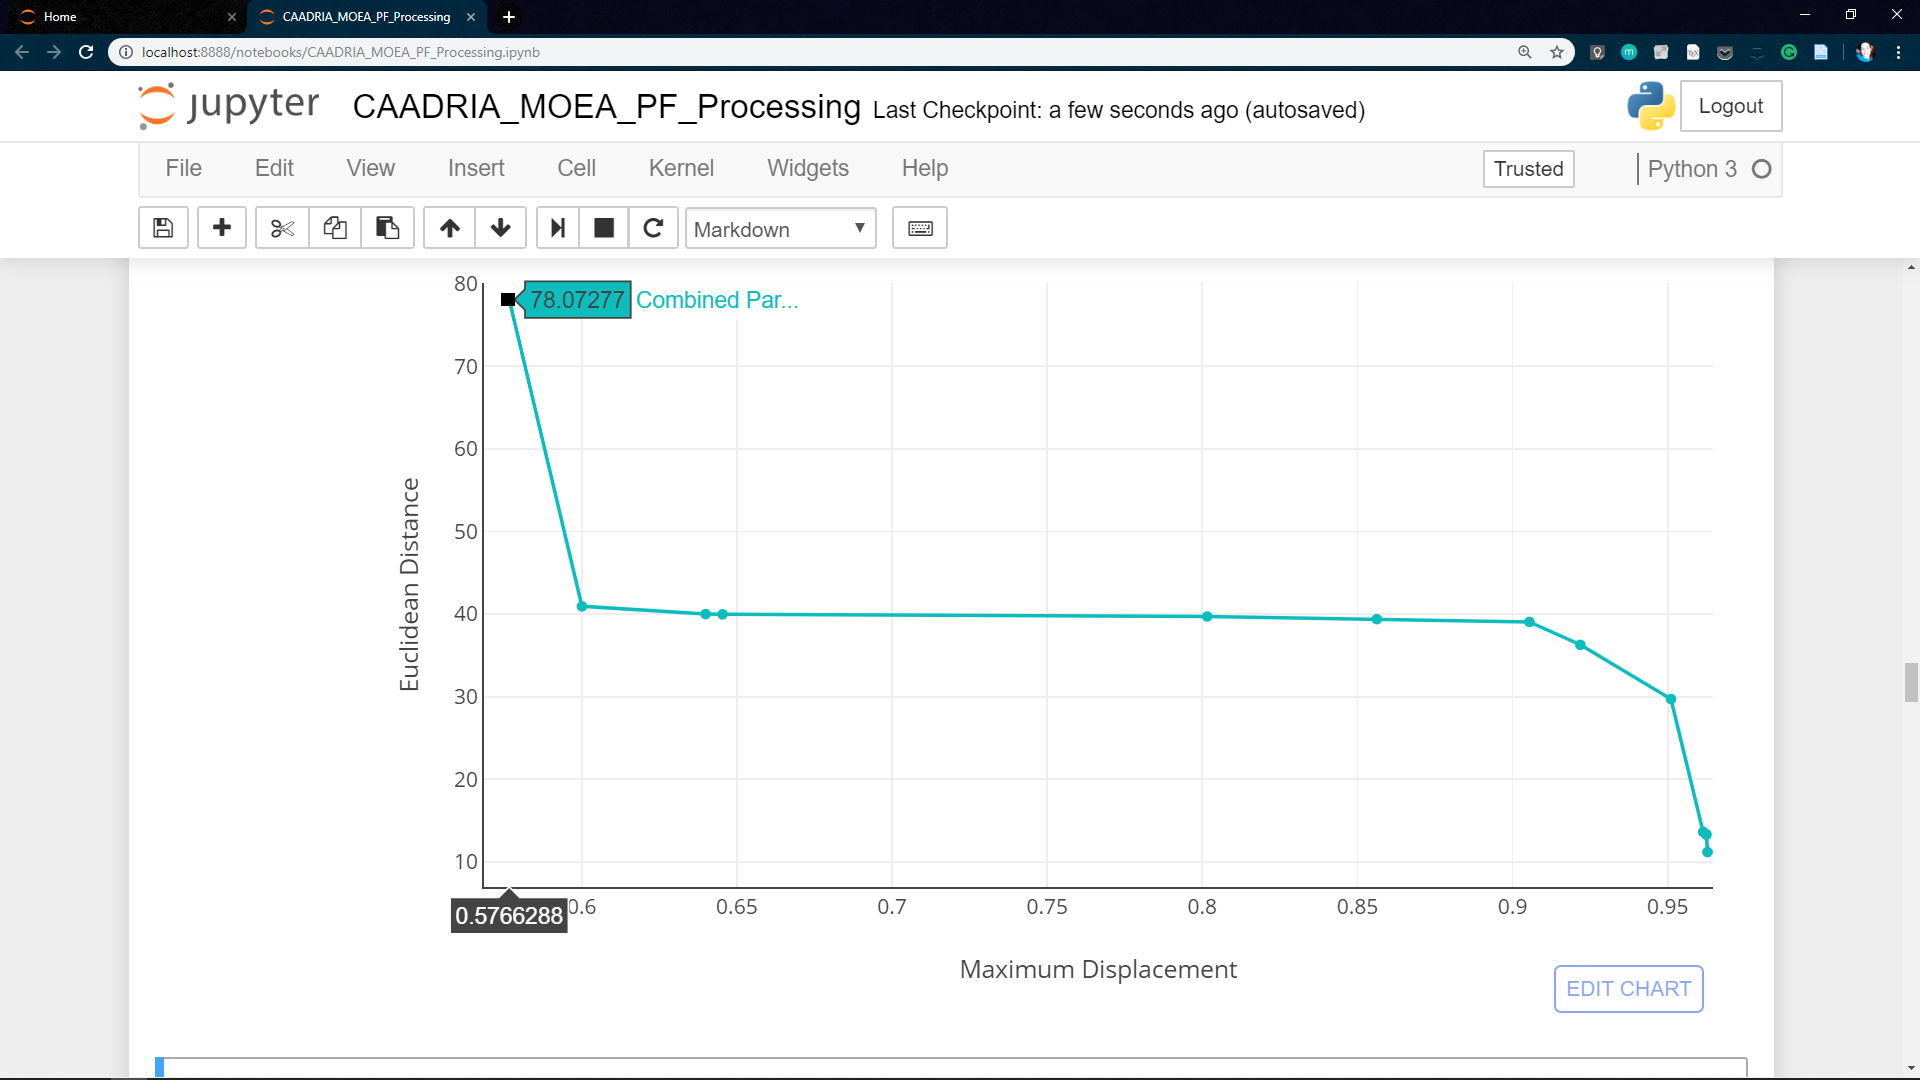
\includegraphics[width=0.625\textwidth]{./Images/Solution/fake-plot-browserview-square.PNG}
	\hfill
	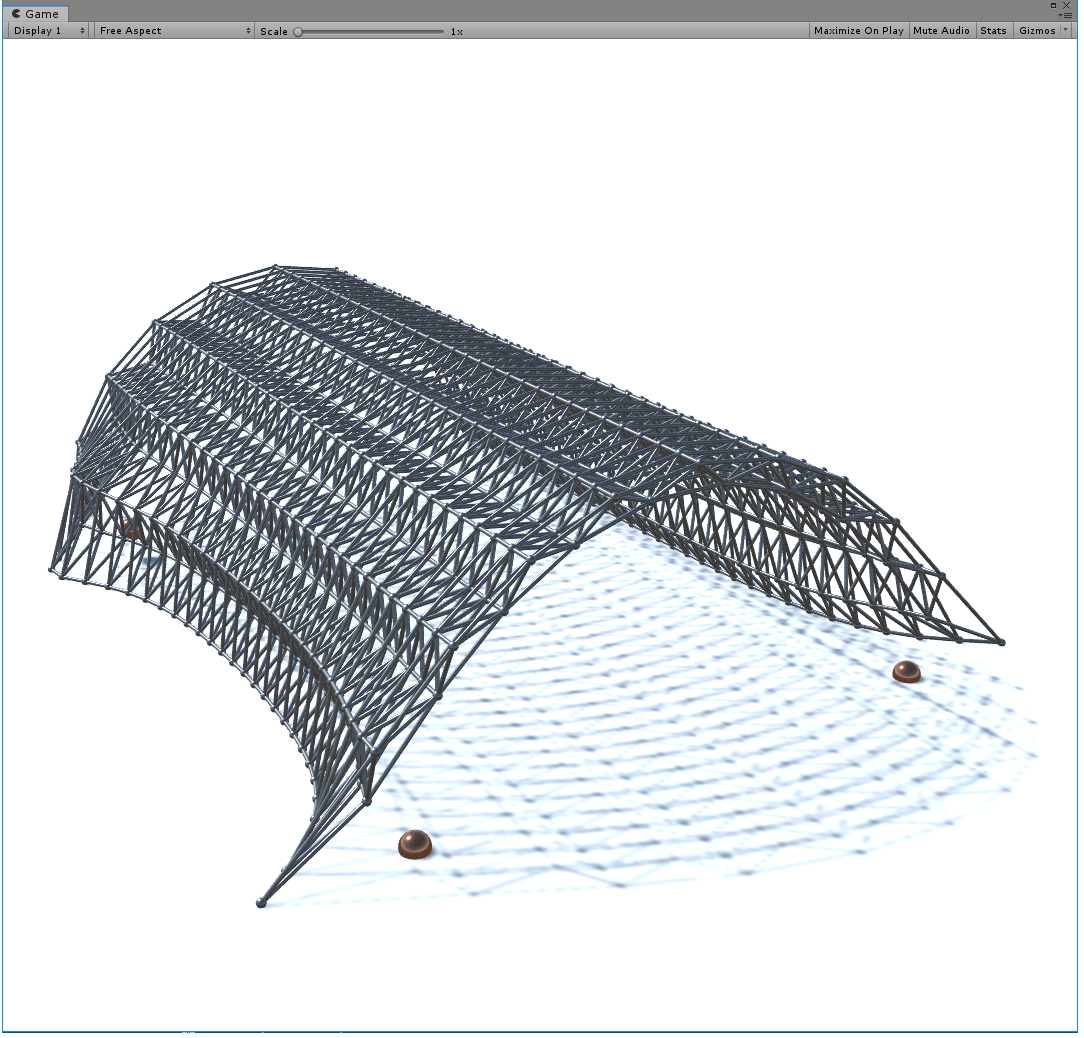
\includegraphics[width=0.365\textwidth]{./Images/Solution/solution3-unity.png}
	
	\caption[Interactive Visualization of Optimization results]{Example of the interactive feature of the proposed optimization framework: on the left, the architect selects one optimal solution, represented with a black square, and the corresponding design's parameters of that solution are used to generate a 3D model, in this case in Unity.}
	\label{fig:interactivefeature}
\end{figure*}
